% Created by tikzDevice version 0.6.2-92-0ad2792 on 2013-03-28 13:04:04
% !TEX encoding = UTF-8 Unicode
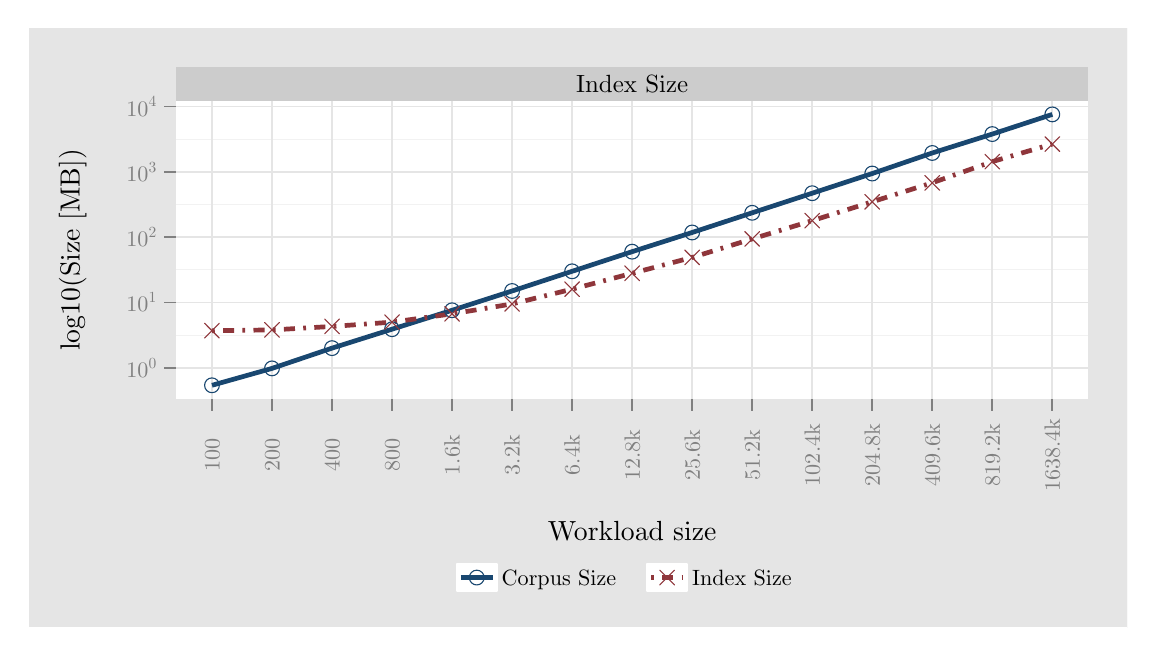
\begin{tikzpicture}[x=1pt,y=1pt]
\definecolor[named]{fillColor}{rgb}{1.00,1.00,1.00}
\path[use as bounding box,fill=fillColor,fill opacity=0.00] (0,0) rectangle (397.48,216.81);
\begin{scope}
\path[clip] (  0.00,  0.00) rectangle (397.48,216.81);
\definecolor[named]{drawColor}{rgb}{1.00,1.00,1.00}
\definecolor[named]{fillColor}{rgb}{0.90,0.90,0.90}

\path[draw=drawColor,line width= 0.6pt,line join=round,line cap=round,fill=fillColor] (  0.00,  0.00) rectangle (397.48,216.81);
\end{scope}
\begin{scope}
\path[clip] ( 53.58, 82.69) rectangle (383.26,190.36);
\definecolor[named]{fillColor}{rgb}{1.00,1.00,1.00}

\path[fill=fillColor] ( 53.58, 82.69) rectangle (383.26,190.36);
\definecolor[named]{drawColor}{rgb}{0.95,0.95,0.95}

\path[draw=drawColor,line width= 0.3pt,line join=round] ( 53.58,105.70) --
	(383.26,105.70);

\path[draw=drawColor,line width= 0.3pt,line join=round] ( 53.58,129.31) --
	(383.26,129.31);

\path[draw=drawColor,line width= 0.3pt,line join=round] ( 53.58,152.91) --
	(383.26,152.91);

\path[draw=drawColor,line width= 0.3pt,line join=round] ( 53.58,176.51) --
	(383.26,176.51);
\definecolor[named]{drawColor}{rgb}{0.90,0.90,0.90}

\path[draw=drawColor,line width= 0.6pt,line join=round] ( 53.58, 93.90) --
	(383.26, 93.90);

\path[draw=drawColor,line width= 0.6pt,line join=round] ( 53.58,117.50) --
	(383.26,117.50);

\path[draw=drawColor,line width= 0.6pt,line join=round] ( 53.58,141.11) --
	(383.26,141.11);

\path[draw=drawColor,line width= 0.6pt,line join=round] ( 53.58,164.71) --
	(383.26,164.71);

\path[draw=drawColor,line width= 0.6pt,line join=round] ( 53.58,188.31) --
	(383.26,188.31);

\path[draw=drawColor,line width= 0.6pt,line join=round] ( 66.60, 82.69) --
	( 66.60,190.36);

\path[draw=drawColor,line width= 0.6pt,line join=round] ( 88.29, 82.69) --
	( 88.29,190.36);

\path[draw=drawColor,line width= 0.6pt,line join=round] (109.97, 82.69) --
	(109.97,190.36);

\path[draw=drawColor,line width= 0.6pt,line join=round] (131.66, 82.69) --
	(131.66,190.36);

\path[draw=drawColor,line width= 0.6pt,line join=round] (153.35, 82.69) --
	(153.35,190.36);

\path[draw=drawColor,line width= 0.6pt,line join=round] (175.04, 82.69) --
	(175.04,190.36);

\path[draw=drawColor,line width= 0.6pt,line join=round] (196.73, 82.69) --
	(196.73,190.36);

\path[draw=drawColor,line width= 0.6pt,line join=round] (218.42, 82.69) --
	(218.42,190.36);

\path[draw=drawColor,line width= 0.6pt,line join=round] (240.11, 82.69) --
	(240.11,190.36);

\path[draw=drawColor,line width= 0.6pt,line join=round] (261.80, 82.69) --
	(261.80,190.36);

\path[draw=drawColor,line width= 0.6pt,line join=round] (283.49, 82.69) --
	(283.49,190.36);

\path[draw=drawColor,line width= 0.6pt,line join=round] (305.18, 82.69) --
	(305.18,190.36);

\path[draw=drawColor,line width= 0.6pt,line join=round] (326.87, 82.69) --
	(326.87,190.36);

\path[draw=drawColor,line width= 0.6pt,line join=round] (348.56, 82.69) --
	(348.56,190.36);

\path[draw=drawColor,line width= 0.6pt,line join=round] (370.25, 82.69) --
	(370.25,190.36);
\definecolor[named]{drawColor}{rgb}{0.10,0.28,0.44}

\path[draw=drawColor,line width= 1.7pt,line join=round] ( 66.60, 87.58) --
	( 88.29, 93.69) --
	(109.97,101.01) --
	(131.66,107.85) --
	(153.35,114.69) --
	(175.04,121.66) --
	(196.73,128.77) --
	(218.42,135.87) --
	(240.11,142.80) --
	(261.80,149.91) --
	(283.49,156.99) --
	(305.18,164.10) --
	(326.87,171.53) --
	(348.56,178.36) --
	(370.25,185.47);
\definecolor[named]{drawColor}{rgb}{0.56,0.21,0.23}

\path[draw=drawColor,line width= 1.7pt,dash pattern=on 1pt off 3pt on 4pt off 3pt ,line join=round] ( 66.60,107.31) --
	( 88.29,107.59) --
	(109.97,108.85) --
	(131.66,110.40) --
	(153.35,113.40) --
	(175.04,116.98) --
	(196.73,122.32) --
	(218.42,128.06) --
	(240.11,133.79) --
	(261.80,140.47) --
	(283.49,147.07) --
	(305.18,153.89) --
	(326.87,160.76) --
	(348.56,168.40) --
	(370.25,174.75);
\definecolor[named]{drawColor}{rgb}{0.10,0.28,0.44}

\path[draw=drawColor,line width= 0.4pt,line join=round,line cap=round] ( 66.60, 87.58) circle (  2.67);

\path[draw=drawColor,line width= 0.4pt,line join=round,line cap=round] ( 88.29, 93.69) circle (  2.67);

\path[draw=drawColor,line width= 0.4pt,line join=round,line cap=round] (109.97,101.01) circle (  2.67);

\path[draw=drawColor,line width= 0.4pt,line join=round,line cap=round] (131.66,107.85) circle (  2.67);

\path[draw=drawColor,line width= 0.4pt,line join=round,line cap=round] (153.35,114.69) circle (  2.67);

\path[draw=drawColor,line width= 0.4pt,line join=round,line cap=round] (175.04,121.66) circle (  2.67);

\path[draw=drawColor,line width= 0.4pt,line join=round,line cap=round] (196.73,128.77) circle (  2.67);

\path[draw=drawColor,line width= 0.4pt,line join=round,line cap=round] (218.42,135.87) circle (  2.67);

\path[draw=drawColor,line width= 0.4pt,line join=round,line cap=round] (240.11,142.80) circle (  2.67);

\path[draw=drawColor,line width= 0.4pt,line join=round,line cap=round] (261.80,149.91) circle (  2.67);

\path[draw=drawColor,line width= 0.4pt,line join=round,line cap=round] (283.49,156.99) circle (  2.67);

\path[draw=drawColor,line width= 0.4pt,line join=round,line cap=round] (305.18,164.10) circle (  2.67);

\path[draw=drawColor,line width= 0.4pt,line join=round,line cap=round] (326.87,171.53) circle (  2.67);

\path[draw=drawColor,line width= 0.4pt,line join=round,line cap=round] (348.56,178.36) circle (  2.67);

\path[draw=drawColor,line width= 0.4pt,line join=round,line cap=round] (370.25,185.47) circle (  2.67);
\definecolor[named]{drawColor}{rgb}{0.56,0.21,0.23}

\path[draw=drawColor,line width= 0.4pt,line join=round,line cap=round,fill=fillColor] ( 63.93,104.64) -- ( 69.26,109.98);

\path[draw=drawColor,line width= 0.4pt,line join=round,line cap=round,fill=fillColor] ( 63.93,109.98) -- ( 69.26,104.64);

\path[draw=drawColor,line width= 0.4pt,line join=round,line cap=round,fill=fillColor] ( 85.62,104.92) -- ( 90.95,110.25);

\path[draw=drawColor,line width= 0.4pt,line join=round,line cap=round,fill=fillColor] ( 85.62,110.25) -- ( 90.95,104.92);

\path[draw=drawColor,line width= 0.4pt,line join=round,line cap=round,fill=fillColor] (107.31,106.19) -- (112.64,111.52);

\path[draw=drawColor,line width= 0.4pt,line join=round,line cap=round,fill=fillColor] (107.31,111.52) -- (112.64,106.19);

\path[draw=drawColor,line width= 0.4pt,line join=round,line cap=round,fill=fillColor] (129.00,107.73) -- (134.33,113.07);

\path[draw=drawColor,line width= 0.4pt,line join=round,line cap=round,fill=fillColor] (129.00,113.07) -- (134.33,107.73);

\path[draw=drawColor,line width= 0.4pt,line join=round,line cap=round,fill=fillColor] (150.69,110.73) -- (156.02,116.07);

\path[draw=drawColor,line width= 0.4pt,line join=round,line cap=round,fill=fillColor] (150.69,116.07) -- (156.02,110.73);

\path[draw=drawColor,line width= 0.4pt,line join=round,line cap=round,fill=fillColor] (172.37,114.31) -- (177.71,119.65);

\path[draw=drawColor,line width= 0.4pt,line join=round,line cap=round,fill=fillColor] (172.37,119.65) -- (177.71,114.31);

\path[draw=drawColor,line width= 0.4pt,line join=round,line cap=round,fill=fillColor] (194.06,119.65) -- (199.40,124.99);

\path[draw=drawColor,line width= 0.4pt,line join=round,line cap=round,fill=fillColor] (194.06,124.99) -- (199.40,119.65);

\path[draw=drawColor,line width= 0.4pt,line join=round,line cap=round,fill=fillColor] (215.75,125.39) -- (221.09,130.73);

\path[draw=drawColor,line width= 0.4pt,line join=round,line cap=round,fill=fillColor] (215.75,130.73) -- (221.09,125.39);

\path[draw=drawColor,line width= 0.4pt,line join=round,line cap=round,fill=fillColor] (237.44,131.13) -- (242.78,136.46);

\path[draw=drawColor,line width= 0.4pt,line join=round,line cap=round,fill=fillColor] (237.44,136.46) -- (242.78,131.13);

\path[draw=drawColor,line width= 0.4pt,line join=round,line cap=round,fill=fillColor] (259.13,137.80) -- (264.47,143.14);

\path[draw=drawColor,line width= 0.4pt,line join=round,line cap=round,fill=fillColor] (259.13,143.14) -- (264.47,137.80);

\path[draw=drawColor,line width= 0.4pt,line join=round,line cap=round,fill=fillColor] (280.82,144.41) -- (286.16,149.74);

\path[draw=drawColor,line width= 0.4pt,line join=round,line cap=round,fill=fillColor] (280.82,149.74) -- (286.16,144.41);

\path[draw=drawColor,line width= 0.4pt,line join=round,line cap=round,fill=fillColor] (302.51,151.22) -- (307.84,156.56);

\path[draw=drawColor,line width= 0.4pt,line join=round,line cap=round,fill=fillColor] (302.51,156.56) -- (307.84,151.22);

\path[draw=drawColor,line width= 0.4pt,line join=round,line cap=round,fill=fillColor] (324.20,158.09) -- (329.53,163.42);

\path[draw=drawColor,line width= 0.4pt,line join=round,line cap=round,fill=fillColor] (324.20,163.42) -- (329.53,158.09);

\path[draw=drawColor,line width= 0.4pt,line join=round,line cap=round,fill=fillColor] (345.89,165.73) -- (351.22,171.07);

\path[draw=drawColor,line width= 0.4pt,line join=round,line cap=round,fill=fillColor] (345.89,171.07) -- (351.22,165.73);

\path[draw=drawColor,line width= 0.4pt,line join=round,line cap=round,fill=fillColor] (367.58,172.08) -- (372.91,177.41);

\path[draw=drawColor,line width= 0.4pt,line join=round,line cap=round,fill=fillColor] (367.58,177.41) -- (372.91,172.08);
\end{scope}
\begin{scope}
\path[clip] (  0.00,  0.00) rectangle (397.48,216.81);
\definecolor[named]{fillColor}{rgb}{0.80,0.80,0.80}

\path[fill=fillColor] ( 53.58,190.36) rectangle (383.26,202.58);
\definecolor[named]{drawColor}{rgb}{0.00,0.00,0.00}

\node[text=drawColor,anchor=base,inner sep=0pt, outer sep=0pt, scale=  0.90] at (218.42,193.37) {Index Size};
\end{scope}
\begin{scope}
\path[clip] (  0.00,  0.00) rectangle (397.48,216.81);
\definecolor[named]{drawColor}{rgb}{0.50,0.50,0.50}

\node[text=drawColor,anchor=base west,inner sep=0pt, outer sep=0pt, scale=  0.80] at ( 35.67, 90.47) {10};

\node[text=drawColor,anchor=base west,inner sep=0pt, outer sep=0pt, scale=  0.56] at ( 43.67, 93.74) {0};

\node[text=drawColor,anchor=base west,inner sep=0pt, outer sep=0pt, scale=  0.80] at ( 35.67,114.07) {10};

\node[text=drawColor,anchor=base west,inner sep=0pt, outer sep=0pt, scale=  0.56] at ( 43.67,117.34) {1};

\node[text=drawColor,anchor=base west,inner sep=0pt, outer sep=0pt, scale=  0.80] at ( 35.67,137.67) {10};

\node[text=drawColor,anchor=base west,inner sep=0pt, outer sep=0pt, scale=  0.56] at ( 43.67,140.95) {2};

\node[text=drawColor,anchor=base west,inner sep=0pt, outer sep=0pt, scale=  0.80] at ( 35.67,161.28) {10};

\node[text=drawColor,anchor=base west,inner sep=0pt, outer sep=0pt, scale=  0.56] at ( 43.67,164.55) {3};

\node[text=drawColor,anchor=base west,inner sep=0pt, outer sep=0pt, scale=  0.80] at ( 35.67,184.88) {10};

\node[text=drawColor,anchor=base west,inner sep=0pt, outer sep=0pt, scale=  0.56] at ( 43.67,188.15) {4};
\end{scope}
\begin{scope}
\path[clip] (  0.00,  0.00) rectangle (397.48,216.81);
\definecolor[named]{drawColor}{rgb}{0.50,0.50,0.50}

\path[draw=drawColor,line width= 0.6pt,line join=round] ( 49.31, 93.90) --
	( 53.58, 93.90);

\path[draw=drawColor,line width= 0.6pt,line join=round] ( 49.31,117.50) --
	( 53.58,117.50);

\path[draw=drawColor,line width= 0.6pt,line join=round] ( 49.31,141.11) --
	( 53.58,141.11);

\path[draw=drawColor,line width= 0.6pt,line join=round] ( 49.31,164.71) --
	( 53.58,164.71);

\path[draw=drawColor,line width= 0.6pt,line join=round] ( 49.31,188.31) --
	( 53.58,188.31);
\end{scope}
\begin{scope}
\path[clip] (  0.00,  0.00) rectangle (397.48,216.81);
\definecolor[named]{drawColor}{rgb}{0.50,0.50,0.50}

\path[draw=drawColor,line width= 0.6pt,line join=round] ( 66.60, 78.42) --
	( 66.60, 82.69);

\path[draw=drawColor,line width= 0.6pt,line join=round] ( 88.29, 78.42) --
	( 88.29, 82.69);

\path[draw=drawColor,line width= 0.6pt,line join=round] (109.97, 78.42) --
	(109.97, 82.69);

\path[draw=drawColor,line width= 0.6pt,line join=round] (131.66, 78.42) --
	(131.66, 82.69);

\path[draw=drawColor,line width= 0.6pt,line join=round] (153.35, 78.42) --
	(153.35, 82.69);

\path[draw=drawColor,line width= 0.6pt,line join=round] (175.04, 78.42) --
	(175.04, 82.69);

\path[draw=drawColor,line width= 0.6pt,line join=round] (196.73, 78.42) --
	(196.73, 82.69);

\path[draw=drawColor,line width= 0.6pt,line join=round] (218.42, 78.42) --
	(218.42, 82.69);

\path[draw=drawColor,line width= 0.6pt,line join=round] (240.11, 78.42) --
	(240.11, 82.69);

\path[draw=drawColor,line width= 0.6pt,line join=round] (261.80, 78.42) --
	(261.80, 82.69);

\path[draw=drawColor,line width= 0.6pt,line join=round] (283.49, 78.42) --
	(283.49, 82.69);

\path[draw=drawColor,line width= 0.6pt,line join=round] (305.18, 78.42) --
	(305.18, 82.69);

\path[draw=drawColor,line width= 0.6pt,line join=round] (326.87, 78.42) --
	(326.87, 82.69);

\path[draw=drawColor,line width= 0.6pt,line join=round] (348.56, 78.42) --
	(348.56, 82.69);

\path[draw=drawColor,line width= 0.6pt,line join=round] (370.25, 78.42) --
	(370.25, 82.69);
\end{scope}
\begin{scope}
\path[clip] (  0.00,  0.00) rectangle (397.48,216.81);
\definecolor[named]{drawColor}{rgb}{0.50,0.50,0.50}

\node[text=drawColor,rotate= 90.00,anchor=base,inner sep=0pt, outer sep=0pt, scale=  0.80] at ( 69.35, 62.36) {100};

\node[text=drawColor,rotate= 90.00,anchor=base,inner sep=0pt, outer sep=0pt, scale=  0.80] at ( 91.04, 62.36) {200};

\node[text=drawColor,rotate= 90.00,anchor=base,inner sep=0pt, outer sep=0pt, scale=  0.80] at (112.73, 62.36) {400};

\node[text=drawColor,rotate= 90.00,anchor=base,inner sep=0pt, outer sep=0pt, scale=  0.80] at (134.42, 62.36) {800};

\node[text=drawColor,rotate= 90.00,anchor=base,inner sep=0pt, outer sep=0pt, scale=  0.80] at (156.11, 62.36) {1.6k};

\node[text=drawColor,rotate= 90.00,anchor=base,inner sep=0pt, outer sep=0pt, scale=  0.80] at (177.80, 62.36) {3.2k};

\node[text=drawColor,rotate= 90.00,anchor=base,inner sep=0pt, outer sep=0pt, scale=  0.80] at (199.49, 62.36) {6.4k};

\node[text=drawColor,rotate= 90.00,anchor=base,inner sep=0pt, outer sep=0pt, scale=  0.80] at (221.18, 62.36) {12.8k};

\node[text=drawColor,rotate= 90.00,anchor=base,inner sep=0pt, outer sep=0pt, scale=  0.80] at (242.86, 62.36) {25.6k};

\node[text=drawColor,rotate= 90.00,anchor=base,inner sep=0pt, outer sep=0pt, scale=  0.80] at (264.55, 62.36) {51.2k};

\node[text=drawColor,rotate= 90.00,anchor=base,inner sep=0pt, outer sep=0pt, scale=  0.80] at (286.24, 62.36) {102.4k};

\node[text=drawColor,rotate= 90.00,anchor=base,inner sep=0pt, outer sep=0pt, scale=  0.80] at (307.93, 62.36) {204.8k};

\node[text=drawColor,rotate= 90.00,anchor=base,inner sep=0pt, outer sep=0pt, scale=  0.80] at (329.62, 62.36) {409.6k};

\node[text=drawColor,rotate= 90.00,anchor=base,inner sep=0pt, outer sep=0pt, scale=  0.80] at (351.31, 62.36) {819.2k};

\node[text=drawColor,rotate= 90.00,anchor=base,inner sep=0pt, outer sep=0pt, scale=  0.80] at (373.00, 62.36) {1638.4k};
\end{scope}
\begin{scope}
\path[clip] (  0.00,  0.00) rectangle (397.48,216.81);
\definecolor[named]{drawColor}{rgb}{0.00,0.00,0.00}

\node[text=drawColor,anchor=base,inner sep=0pt, outer sep=0pt, scale=  1.00] at (218.42, 31.41) {Workload size};
\end{scope}
\begin{scope}
\path[clip] (  0.00,  0.00) rectangle (397.48,216.81);
\definecolor[named]{drawColor}{rgb}{0.00,0.00,0.00}

\node[text=drawColor,rotate= 90.00,anchor=base,inner sep=0pt, outer sep=0pt, scale=  1.00] at ( 18.80,136.53) {log10(Size [MB])};
\end{scope}
\begin{scope}
\path[clip] (  0.00,  0.00) rectangle (397.48,216.81);
\definecolor[named]{fillColor}{rgb}{0.90,0.90,0.90}

\path[fill=fillColor] (147.16,  8.87) rectangle (289.68, 27.36);
\end{scope}
\begin{scope}
\path[clip] (  0.00,  0.00) rectangle (397.48,216.81);
\definecolor[named]{drawColor}{rgb}{1.00,1.00,1.00}
\definecolor[named]{fillColor}{rgb}{1.00,1.00,1.00}

\path[draw=drawColor,line width= 0.6pt,line join=round,line cap=round,fill=fillColor] (155.04, 13.14) rectangle (169.49, 23.09);
\end{scope}
\begin{scope}
\path[clip] (  0.00,  0.00) rectangle (397.48,216.81);
\definecolor[named]{drawColor}{rgb}{0.10,0.28,0.44}

\path[draw=drawColor,line width= 1.7pt,line join=round] (156.49, 18.11) -- (168.05, 18.11);
\end{scope}
\begin{scope}
\path[clip] (  0.00,  0.00) rectangle (397.48,216.81);
\definecolor[named]{drawColor}{rgb}{0.10,0.28,0.44}

\path[draw=drawColor,line width= 0.4pt,line join=round,line cap=round] (162.27, 18.11) circle (  2.67);
\end{scope}
\begin{scope}
\path[clip] (  0.00,  0.00) rectangle (397.48,216.81);
\definecolor[named]{drawColor}{rgb}{1.00,1.00,1.00}
\definecolor[named]{fillColor}{rgb}{1.00,1.00,1.00}

\path[draw=drawColor,line width= 0.6pt,line join=round,line cap=round,fill=fillColor] (223.83, 13.14) rectangle (238.28, 23.09);
\end{scope}
\begin{scope}
\path[clip] (  0.00,  0.00) rectangle (397.48,216.81);
\definecolor[named]{drawColor}{rgb}{0.56,0.21,0.23}

\path[draw=drawColor,line width= 1.7pt,dash pattern=on 1pt off 3pt on 4pt off 3pt ,line join=round] (225.28, 18.11) -- (236.84, 18.11);
\end{scope}
\begin{scope}
\path[clip] (  0.00,  0.00) rectangle (397.48,216.81);
\definecolor[named]{drawColor}{rgb}{0.56,0.21,0.23}
\definecolor[named]{fillColor}{rgb}{1.00,1.00,1.00}

\path[draw=drawColor,line width= 0.4pt,line join=round,line cap=round,fill=fillColor] (228.39, 15.45) -- (233.72, 20.78);

\path[draw=drawColor,line width= 0.4pt,line join=round,line cap=round,fill=fillColor] (228.39, 20.78) -- (233.72, 15.45);
\end{scope}
\begin{scope}
\path[clip] (  0.00,  0.00) rectangle (397.48,216.81);
\definecolor[named]{drawColor}{rgb}{0.00,0.00,0.00}

\node[text=drawColor,anchor=base west,inner sep=0pt, outer sep=0pt, scale=  0.80] at (171.30, 15.36) {Corpus Size $\;\;\;$};
\end{scope}
\begin{scope}
\path[clip] (  0.00,  0.00) rectangle (397.48,216.81);
\definecolor[named]{drawColor}{rgb}{0.00,0.00,0.00}

\node[text=drawColor,anchor=base west,inner sep=0pt, outer sep=0pt, scale=  0.80] at (240.09, 15.36) {Index Size $\;\;\;$};
\end{scope}
\end{tikzpicture}
